\documentclass[a4paper]{article}
\usepackage{graphicx} % Required for inserting images
\usepackage{amssymb}
\usepackage{amsmath}
\usepackage{amsthm}
\usepackage{hyperref}
\usepackage{listings}
\usepackage{fancyhdr}
\usepackage[table]{xcolor}
\usepackage{geometry}
\usepackage{ragged2e}
\usepackage{subcaption}
\usepackage{multirow}
\usepackage{tabularx}
\usepackage{indentfirst}
\usepackage{lscape}
\usepackage{titlesec}
\usepackage[nottoc,numbib]{tocbibind}
\usepackage[usenames, dvipsnames]{xcolor}
\usepackage{tikz} \usetikzlibrary{calc}
%\usepackage[boxed, linesnumbered]{algorithm2e}
\usepackage{algpseudocode}
\usepackage{algorithm}


\geometry{margin=1in}

\colorlet{myGreen}{green!70!black}
\colorlet{myDGreen}{green!50!black}
\colorlet{myGray}{white!90!black}

%\newcommand{\colNaN}[1]{{\textcolor{black!30}{#1}}}
%\newcommand{\colDisaster}[1]{{\textcolor{red!60}{#1}}}
%\newcommand{\colFailure}[1]{{\textcolor{orange}{#1}}}
%\newcommand{\colWorse}[1]{\textcolor{orange!60}{#1}}
%\newcommand{\colSimilar}[1]{\textcolor{black!60}{#1}}
%\newcommand{\colBetter}[1]{\textcolor{blue!70}{#1}}
%\newcommand{\colSuccess}[1]{\textcolor{black!30!green}{#1}}
%\newcommand{\colAmazing}[1]{\textcolor{green}{#1}}

\hypersetup{
    colorlinks,
    linkcolor={blue!50!black},
    citecolor={blue!50!black},
    urlcolor={blue!80!black}
}

\lstdefinestyle{mystyle}{
    language=Python,
    backgroundcolor=\color{white!95!black},   
    %commentstyle=\color{},
    %keywordstyle=\color{},
    %numberstyle=\tiny\color{codegray},
    %stringstyle=\color{codepurple},
    basicstyle=\ttfamily\footnotesize,
    breakatwhitespace=false,         
    breaklines=true,                 
    %captionpos=b,                    
    keepspaces=true,                 
    %numbers=left,                    
    %numbersep=5pt,                  
    showspaces=false,                
    showstringspaces=false,
    showtabs=false,                  
    tabsize=4,
}
\lstset{
    style=mystyle,
    %emph={sage},
    %emphstyle={\color{myGreen}}
}



%\renewcommand\footnoterule{\rule{.4\textwidth}{0.2pt}}
\renewcommand\footnoterule{\kern-3pt \hrule  \kern 2.6pt}
\fancyhead[L, C]{}
\fancyfoot[C]{\thepage}
\pagestyle{fancy}

\newtheorem{theorem}{Theorem}
\newtheorem{proposition}[theorem]{Proposition}

\newtheorem*{remark}{Remark}

\theoremstyle{definition}
\newtheorem{definition}{Definition}
\newtheorem*{example}{Example}


\begin{document}

\thispagestyle{plain}
\begin{titlepage}
    \begin{figure}[h]
        \centering
        \includegraphics[width=0.4\textwidth]{su.png}
    \end{figure}
    \vspace{1cm}

    \begin{center}
        {\LARGE PCCA}\\[0.3cm]
        \rule{\linewidth}{0.5mm} \\[0.4cm]
        {\huge \textbf{Arithmétique modulaire et vectorisation\\ SIMD / AVX}}\\[0.4cm]
        \rule{\linewidth}{0.5mm} \\[1cm]
        {\large 24 January 2025 - ?? May 2025}\\[3cm]

        {\Large Damien ASSIRE \& Marie BONBOIRE}


    \end{center}

    \vfill
\begin{flushleft}{\large
    \textbf{Supervisor:} Mr. Vincent NEIGER (LIP6 - PolSys)\\
    }
\end{flushleft}
\end{titlepage}
\newpage

\tableofcontents
\newpage

\section{Preface}

\subsection{Subject}
\subsection{Machines description}


% 2023 - 4.5 GHz % mariz
% 2019 - 2.5 GHz % ppti
% 2023 - 3.3 GHz % argiope
% 2021 - 3.0 GHz % groebner

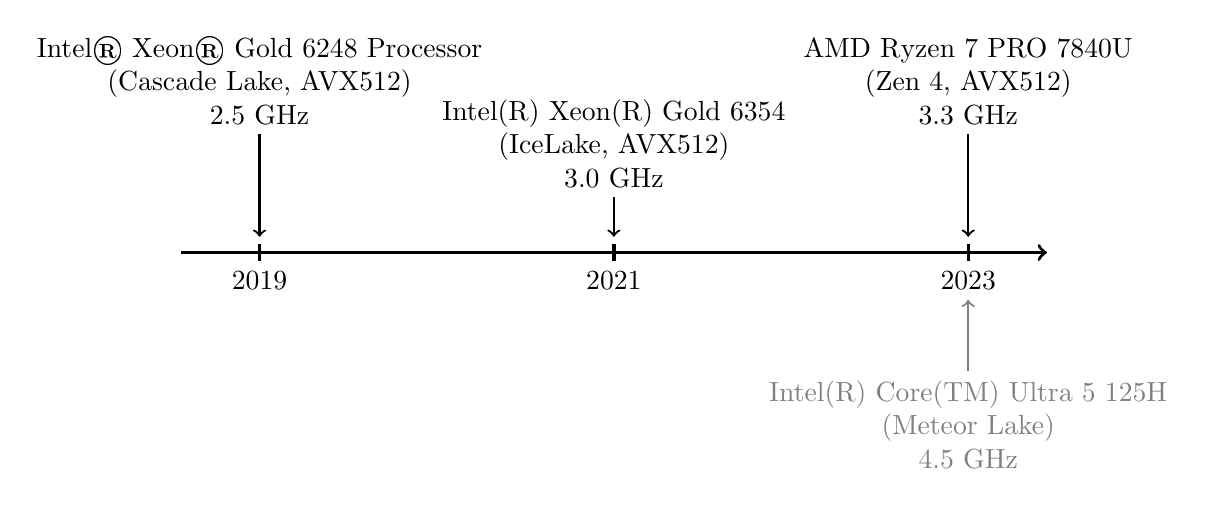
\begin{tikzpicture}[very thick, black]

    %coordinates
    \coordinate (O) at (1,0); % Origin
    \coordinate (F) at (12,0); %End
    \coordinate (P1) at (2,0); %ppti
    \coordinate (P2) at (6.5,0); %groebner
    \coordinate (P3) at (11,0); %mariz+argiope

    %proc
    \draw[<-,thick,color=black] ($(P1)+(0,0.2)$) -- ($(P1)+(0,1.5)$) node [above=0pt,align=center,black] 
    {Intel® Xeon® Gold 6248 Processor \\ (Cascade Lake, AVX512) \\ 2.5 GHz};
    \draw[<-,thick,color=black] ($(P2)+(0,0.2)$) -- ($(P2)+(0,0.7)$) node [above=0pt,align=center,black] 
    {Intel(R) Xeon(R) Gold 6354 \\ (IceLake, AVX512) \\ 3.0 GHz};
    \draw[<-,thick,color=black] ($(P3)+(0,0.2)$) -- ($(P3)+(0,1.5)$) node [above=0pt,align=center,black] 
    {AMD Ryzen 7 PRO 7840U \\ (Zen 4, AVX512) \\ 3.3 GHz};
    \draw[<-,thick,color=gray] ($(P3)-(0,0.6)$) -- ($(P3)-(0,1.5)$) node [below=0pt,align=center,gray] 
    {Intel(R) Core(TM) Ultra 5 125H \\ (Meteor Lake) \\ 4.5 GHz};

    %main arrow
    \draw[->] (O) -- (F);

    %ticks
    \foreach \x in {2,6.5,11}
    \draw(\x cm,3pt) -- (\x cm,-3pt);
    %labels
    \foreach \i \j in {2/2019,6.5/2021,11/2023}{
    	\draw (\i,0) node[below=3pt] {\j} ;
    }

\end{tikzpicture}

\section{Bottlenecks}

\subsection{Overflow}
\subsection{Throughput}
\subsection{Modulo}

\section{Profiling/Benchmarking}

\subsection{Impact of caches} % todo Draft

In the benchmarks, we observes bigger factors than expected between two sizes,
e.g. during the unrolling of non modular dot product. This happen when a vector
become too big to fit in a certain cache, and must be stored in a lower level
cache or in the primary memory. In the previously cited case, it happen for sizes
65536 and 131072 on ppti-gpu-4. % todo detail of calculation

\section{Outcome}

\section{Conclusion}

\newpage
\bibliographystyle{plain} 
\bibliography{biblio} 
\nocite{*}

\end{document}
